\documentclass[12pt,]{article}
\usepackage[superscript,nomove]{cite} % use if \cite is used and superscripts wanted
\usepackage[utf8]{inputenc}
\usepackage[a4paper, margin=1.2in]{geometry}
\usepackage{amsmath}
\usepackage{graphicx}
\usepackage{lscape}
\usepackage{bbm}
\usepackage{mathrsfs}
\usepackage{amssymb}
\usepackage{amsmath,amssymb,amsthm}
\usepackage{listings}
\usepackage{color} %red, green, blue, yellow, cyan, magenta, black, white
\usepackage{longtable}
\usepackage{tabularx}
\usepackage{rotating}
\usepackage{fancyhdr}          % this and next line are for fancy headers/footers
\pagestyle{fancy}

\usepackage{Sweavel}

% To produce both postscript and pdf graphics, remove the eps and pdf
% parameters in the next line.  Set default plot size to 6x4 in.

%\SweaveOpts{width=8, height=6}



\begin{document}
\begin{titlepage}
\begin{center}

\vspace*{5em}
{\huge A Production Efficiency Analysis of Farms using the DEA Approach\\[0.4cm] }
\color{blue}\hrule
\color{black}
\vspace{100mm}
\noindent
\Large Jiachuan \textsc{Tian}

\today
\vfill
\end{center}
\end{titlepage}


%--------------------------------
\section{Data Desciption}
%--------------------------------


In this note, we present an analysis of farms' production efficiencies using the DEA approach. The data we use is monthly data of a set of farms. We first checked the number of farms and the number of variates.

\begin{Schunk}
\begin{Sinput}
> data = read.xlsx(file = 'Monthly.xlsx', 1)
> data$Farm_ID = factor(data$Farm_ID)  #Change Farm_ID to Factor
> data %<>%
+   dplyr::distinct() %>%
+   group_by(Farm_ID) %>%
+   arrange(DHIDate)
> dim(data)
\end{Sinput}
\begin{Soutput}
[1] 2303   36
\end{Soutput}
\begin{Sinput}
> length(unique(data$Farm_ID))
\end{Sinput}
\begin{Soutput}
[1] 53
\end{Soutput}
\end{Schunk}
Thus we have 53 farms, 36 variates for each farm. We have a total number of 2346 observations. We suspect there may be some missing values in the data.
\begin{Schunk}
\begin{Sinput}
> missing_fn = function(col_index){
+   return(sum(is.na(data[,col_index])))
+ }
> result = sapply(1:dim(data)[2], function(x) missing_fn(x))
> missing_value = as.data.frame(result)
> missing_value$Var = colnames(data)
> colnames(missing_value)[1] = "Number of Available Observations"
> missing_value = missing_value[, c(2, 1)]
> missing_value[2] = dim(data)[1] - missing_value[2]
> mis_tab = xtable(missing_value,
+                  caption ="Number of Missing Values", 
+                  label = "Table-1")
> align(mis_tab) = "ll|r"
> print(mis_tab, latex.environments = "center", size = .1, 
+       tabular.environment = "longtable")
\end{Sinput}
% latex table generated in R 3.2.2 by xtable 1.8-2 package
% Thu Mar 31 14:23:18 2016
\begin{longtable}{ll|r}
  \hline
 & Var & Number of Available Observations \\ 
  \hline
1 & Farm\_ID & 2303 \\ 
  2 & Herdcode & 2303 \\ 
  3 & Milk\_per\_Milk\_Cow & 2303 \\ 
  4 & X\_\_Fat & 2303 \\ 
  5 & X\_\_Pro & 2303 \\ 
  6 & X\_\_Cows & 2303 \\ 
  7 & ME\_305\_Milk & 2292 \\ 
  8 & ME\_305\_Fat & 2292 \\ 
  9 & ME\_305\_Pro & 2292 \\ 
  10 & X\_\_Milk\_Cows & 2303 \\ 
  11 & X\_50\_D\_Milk & 2303 \\ 
  12 & Peak & 2292 \\ 
  13 & Summit & 2292 \\ 
  14 & DHIDate & 2303 \\ 
  15 & month & 2303 \\ 
  16 & year & 2303 \\ 
  17 & Sample\_Number & 160 \\ 
  18 & Season\_Year & 160 \\ 
  19 & MUN & 159 \\ 
  20 & Dry\_Matter & 160 \\ 
  21 & CP\_\_ & 160 \\ 
  22 & NDF\_\_\_DM & 160 \\ 
  23 & Starch\_\_\_DM & 160 \\ 
  24 & Starch\_Digestibility & 160 \\ 
  25 & NDF\_Digestibility & 125 \\ 
  26 & NDF\_Dig\_Group & 114 \\ 
  27 & Fecal\_Starch & 160 \\ 
  28 & pH & 145 \\ 
  29 & Hybrid &  88 \\ 
  30 & Structure &  88 \\ 
  31 & SampleDate & 160 \\ 
  32 & Parent\_Company &  54 \\ 
  33 & Hybrid\_Company &  56 \\ 
  34 & Hybrid\_Name &  54 \\ 
  35 & Trait &  45 \\ 
  36 & relative\_maturity &  54 \\ 
   \hline
\hline
\caption{Number of Missing Values} 
\label{Table-1}
\end{longtable}\end{Schunk}

Data were drawn from 53 farms on a monthly basis for 2013-2015. During some months, each quarter, we sampled feed, manure, and other performance indicators and conducted tests. We call those months, sampled months, and the additional data collected as test data. Of interest is to determine whether the data collected during the sampled months was generated from the same distribution as that collected in the other months.


\begin{Schunk}
\begin{Sinput}
> sample = data[!is.na(data$Sample_Number), ]
> length(unique(sample$Farm_ID))
\end{Sinput}
\begin{Soutput}
[1] 53
\end{Soutput}
\end{Schunk}
The number of farm in the (sub)sample is the same as that in data. Thus every farm has been sampled. We are good.
 
%------------------------------
\section{Heterogeneity Tests}
%-----------------------------
We suspect there are heterogeneities in two aspects: (i) sample versus nonsample within each farm; (ii) across farms. We first check for each firm, whether the sampled and nonsampled data are generated from the same distribution for each variates. In particular, we use three nonparametric tests(Kruskal Wallis Test, Kolmogorov-Smirnov Test and Wilcoxon Rank Sum Test) to test  heterogneity.


\subsection{Kruskal Wallis Test}
The null hypothesis of Kruskal Wallis Test is:
\begin{center}
$\textbf{\textit{H}}_0$: Two samples tested are generated from the same distribution.
\end{center}
The test statistic of Kruskal Wallis test is 
\begin{align}
H = (N-1) \frac{\sum_{i = 1}^2 n_i (\bar{r}_i- \bar{r})}{\sum_{i=1}^2 \sum_{j = 1}^{n_i} (r_{ij} - \bar{r})}
\end{align}
where $N$ is the total number of observations and $n_i$ is the number of observations in group $i$ for $i = 1, 2$. $r_{ij}$ is the ranking of observation $j$ from group $i$. $\bar{r}_i = \sum_{j = 1}^{n_i} r_{ij} \ n_i$ is the average rank of group $i$. 
Under the null hypothesis, $H \sim \chi^2_1$. Reject the null hypothesis when $H > \chi^2_{\alpha, 1}$.

Table-2 reports the p-value of Kruskal Wallis test of the sample vs nonsample heterogeneity for each variate within each firm. If the p-value is smaller than 0.05, we conclude there is heterogeneity between sampled data and nonsampled data. Otherwise, we conclude they are generated from the same distribution.

%<<Kruskal Wallis Test, results=tex>>=
%kruskal_test_fn = function(Farm_ID, col_index, data){
%  local_sample = data[(!is.na(data$Sample_Number)) & 
%                        data$Farm_ID == Farm_ID, col_index]
%  local_nonsample = data[(is.na(data$Sample_Number)) & 
%                           data$Farm_ID == Farm_ID, col_index]
%  return(kruskal.test(list(local_sample, local_nonsample))
%         $p.value)
%}
%kruskal_test = outer(
%  unique(sample$Farm_ID), 
%  (3:13),
%  Vectorize(function(x, y) kruskal_test_fn(x, y, data))
%)
%kruskal_test = as.data.frame(kruskal_test)
%colnames(kruskal_test) = colnames(data)[3:13]
%kruskal_test$Farm_ID = unique(data$Farm_ID)
%kruskal_test = kruskal_test[,c(12, 1 : 11)]
%ruskal_tab = xtable(kruskal_test, 
%                     caption = "Kruskal Wallis Test", 
%                     label = "Table-2")
%print(kruskal_tab, latex.environments ="center", size ="small", 
%      rotate.colnames = TRUE, tabular.environment = "longtable")
%@
\textbf{Conclusion}: From table-2, we see almost all p-value are bigger than 0.05. Thus we conclude that the sampled data and nonsampled data are generated from the same distribution.



\subsection{Kolmogorov-Smirnov Test}
The null hypothesis of Kolmogorov-Smirnov Test is:
\begin{center}
$\textbf{\textit{H}}_0$: Two samples tested are generated from the same distribution.
\end{center}
The test statistic of Kolmogorov-Smirnov test is:
\begin{align}
D_{n, n'} = \sup_x |F_{1,n}(x) - F_{2,n}(x)|
\end{align}
where $n$ and $n'$ are the number of observations of the two samples. $F_{1,n}$ and $F_{2,n'}$ are the empirical distribution functions of the two samples respectively. Reject the null hypothesis at level $\alpha$ if $D_{n, n'} > c(\alpha) \sqrt{\frac{n + n'}{nn'}}$. $C(\alpha)$ can be found in the critical value table.

Table-3 reports the p-value of Kolmogorov-Smirnov Test of the sample vs nonsample heterogeneity for each variate within each firm. If the p-value is smaller than 0.05, we conclude there is heterogeneity between sampled data and nonsampled data. Otherwise, we conclude they are generated from the same distribution.

%<<Kolmogorov-Smirnov Test, results=tex>>=
%ks_test_fn = function(Farm_ID, col_index, data){
%  local_sample = data[(!is.na(data$Sample_Number)) &
%                        data$Farm_ID == Farm_ID, col_index]
%  local_nonsample = data[(is.na(data$Sample_Number)) &
%                           data$Farm_ID == Farm_ID, col_index]
% return(ks.test(local_sample, local_nonsample)$p.value)
%}
%ks_test = outer(
%  unique(sample$Farm_ID), 
%  (3:13),
%  Vectorize(function(x, y) ks_test_fn(x, y, data))
%)
%ks_test = as.data.frame(ks_test)
%colnames(ks_test) = colnames(data)[3:13]
%ks_test$Farm_ID = unique(data$Farm_ID)
%ks_test = ks_test[,c(12, 1 : 11)]
%ks_tab = xtable(ks_test, 
%                caption = "Kolmogorov-Smirnov Test", 
%                label = "Table-3")
%print(ks_tab, latex.environments = "center", size =  "small", 
%      rotate.colnames = TRUE, tabular.environment = "longtable")
%@
\textbf{Conclusion}: From table-3, we see almost all p-value are bigger than 0.05. Thus we conclude the same as in Kruskal Wallis test.



\subsection{Wilcoxon Rank Sum Test}
The null hypothesis of Wilcoxon Rank Sum Test (equivalently Mann-Whitney test) is:
\begin{center}
$\textbf{\textit{H}}_0$: Two samples tested are generated from the same distribution.
\end{center}
It is worth noting that wilcoxon rank sum test can only test two samples of the same size. Let $N$ be the sample size. The test statistic of Wilcoxon Rank sum test is:
\begin{align}
W = \sum_{i = 1}^{N_r}[sgn(x_{2,i} - x_{1,i}) R_i]
\end{align}
where sgn() is the sign function, $x_{1, i}$ and $x_{2, i}$ are observation of the two samples. $N_r$ is the number excluding the pairs with $|x_{2, i} - x_{1, i}| = 0$. Under the null hypothesis, $W$ follows a specific distribution with no simple expression with 0 expectation and variance of $\frac{N_r(N_r + 1)(2N_r + 1)}{6}$. Reject the null hypothesis if $|W| > W_{critical, N_r}$.


Table-4 reports the p-value of Wilcoxon Rank Sum test of the sample vs nonsample heterogeneity for each variate within each firm. If the p-value is smaller than 0.05, we conclude there is heterogeneity between sampled data and nonsampled data. Otherwise, we conclude they are generated from the same distribution.

%<<Wilcoxon Rank Sum Test, results=tex>>=

%wilcox_test_fn = function(Farm_ID, col_index, data){
%  local_sample = data[(!is.na(data$Sample_Number)) &
%                        data$Farm_ID == Farm_ID, col_index]
%  local_nonsample = data[(is.na(data$Sample_Number)) &
%                           data$Farm_ID == Farm_ID, col_index]
%  return(wilcox.test(local_sample, local_nonsample)$p.value)
%}
%wilcox_test = outer(
%  unique(sample$Farm_ID), 
%  (3:13),
%  Vectorize(function(x, y) wilcox_test_fn(x, y, data))
%)
%wilcox_test = as.data.frame(wilcox_test)
%colnames(wilcox_test) = colnames(data)[3:13]
%wilcox_test$Farm_ID = unique(data$Farm_ID)
%wilcox_test = wilcox_test[,c(12, 1 : 11)]
%wilcox_tab = xtable(wilcox_test, 
%                    caption = "Wilcoxon Rank Sum Test", 
%                    label = "Table-4")
%print(wilcox_tab, latex.environments = "center", size =  "small", 
%      rotate.colnames = TRUE, tabular.environment = "longtable")
%@
\textbf{Conclusion}: From table-4, we see almost all p-value are bigger than 0.05. Thus we conclude that the sampled data and nonsampled data are generated from the same distribution.

\subsection{Heterogeneity Test of Farms}
In this section we examine the herterogeneity of number of milk cows across farms. In particular, we use Kruskal Wallis test to test such heterogeneity.

\begin{Schunk}
\begin{Sinput}
> kruskal.test(data$X__Cows ~ data$Farm_ID)               
\end{Sinput}
\begin{Soutput}
	Kruskal-Wallis rank sum test

data:  data$X__Cows by data$Farm_ID
Kruskal-Wallis chi-squared = 2239.8, df = 52, p-value < 2.2e-16
\end{Soutput}
\end{Schunk}
The p-value is very small. Thus we conclude there is heterogeneity across farms. Figure-1 visualizes the heterogeneity of number of milk cows across farms. 

\begin{Schunk}
\begin{Sinput}
> kruskal.test(data$Milk_per_Milk_Cow ~ data$Farm_ID)
\end{Sinput}
\begin{Soutput}
	Kruskal-Wallis rank sum test

data:  data$Milk_per_Milk_Cow by data$Farm_ID
Kruskal-Wallis chi-squared = 1555.6, df = 52, p-value < 2.2e-16
\end{Soutput}
\end{Schunk}

\begin{figure}[h]
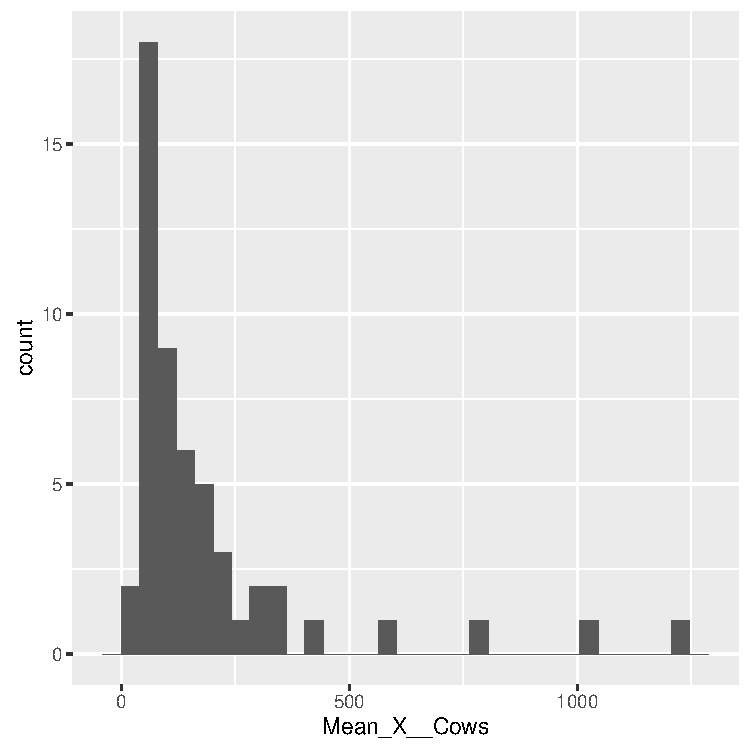
\includegraphics{DEA-Hetero}
\caption{Number of Cows by Farm ID}
\end{figure}


\newpage
%--------------------------
\section{DEA}
%--------------------------
\subsection{Model 1: Single Input, Single Output DEA on Monthly Data}

In this section, we examine the production efficieny of farms. We caculate three input efficiency scores with number of milk cows as input, and milk per milk cow,  fat, pro as outputs respectively. The milk per milk cow efficiency is reported as follows:


\begin{Schunk}
\begin{Sinput}
> summary(dea_Milk)
\end{Sinput}
\begin{Soutput}
Summary of efficiencies
The technology is vrs and input orientated efficiency
Number of firms with efficiency==1 are 6 
Mean efficiency: 0.343 
---                
  Eff range        #     %
  0<= E <0.1     312 13.55
  0.1<= E <0.2   474 20.58
  0.2<= E <0.3   443 19.24
  0.3<= E <0.4   288 12.51
  0.4<= E <0.5   187  8.12
  0.5<= E <0.6   152  6.60
  0.6<= E <0.7   208  9.03
  0.7<= E <0.8   154  6.69
  0.8<= E <0.9    60  2.61
  0.9<= E <1      19  0.83
        E ==1      6  0.26
   Min. 1st Qu.  Median    Mean 3rd Qu.    Max. 
 0.0240  0.1522  0.2828  0.3428  0.5107  1.0000 
\end{Soutput}
\end{Schunk}

\begin{figure}[h]
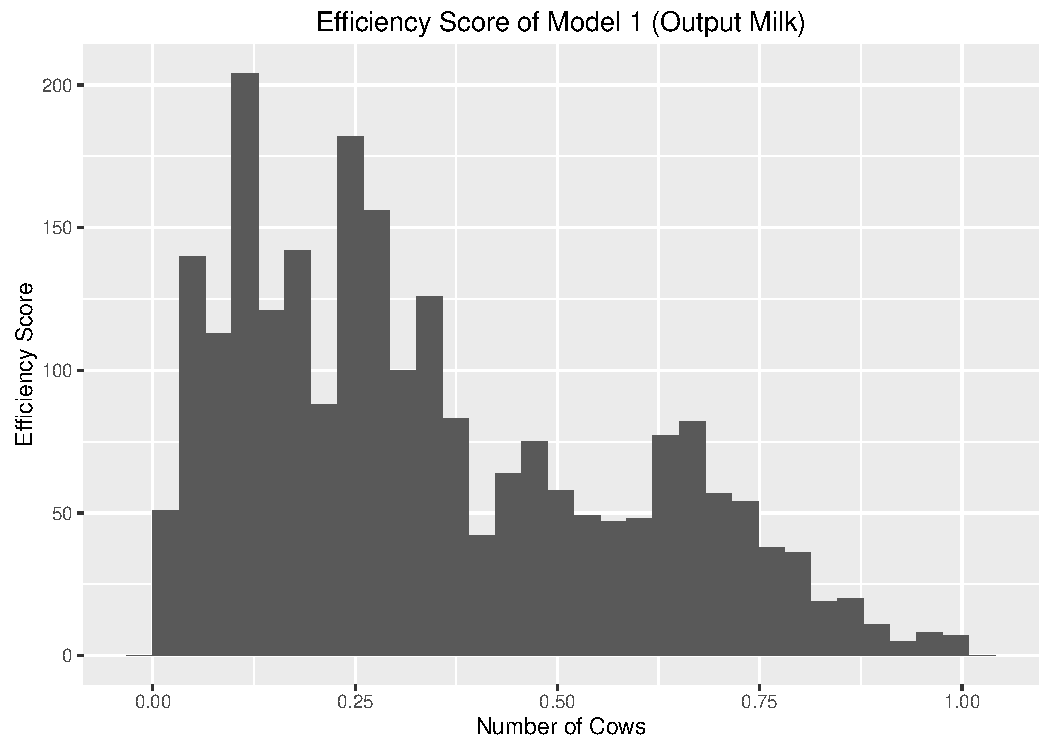
\includegraphics{DEA-DEA_1}
\end{figure}



The milk fat production efficiencies can be summarized as follows:
\begin{Schunk}
\begin{Sinput}
> summary(dea_pro)
\end{Sinput}
\begin{Soutput}
Summary of efficiencies
The technology is vrs and input orientated efficiency
Number of firms with efficiency==1 are 2 
Mean efficiency: 0.31 
---                
  Eff range        #      %
  0<= E <0.1     412 17.890
  0.1<= E <0.2   443 19.236
  0.2<= E <0.3   442 19.192
  0.3<= E <0.4   276 11.984
  0.4<= E <0.5   226  9.813
  0.5<= E <0.6   177  7.686
  0.6<= E <0.7   184  7.990
  0.7<= E <0.8   109  4.733
  0.8<= E <0.9    28  1.216
  0.9<= E <1       4  0.174
        E ==1      2  0.087
   Min. 1st Qu.  Median    Mean 3rd Qu.    Max. 
0.02144 0.13460 0.24560 0.31010 0.46670 1.00000 
\end{Soutput}
\end{Schunk}

\begin{figure}[h]
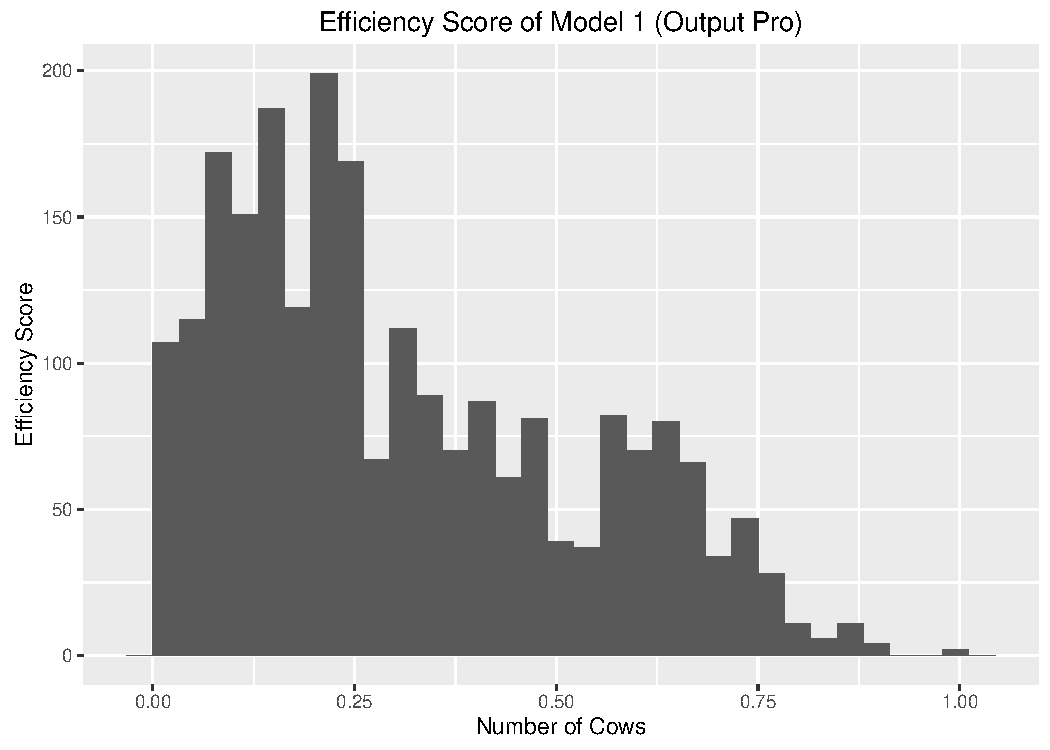
\includegraphics{DEA-DEA_2}
\end{figure}

And the milk protein efficiencies can be summarized  as follows:
\begin{Schunk}
\begin{Sinput}
> summary(dea_fat)
\end{Sinput}
\begin{Soutput}
Summary of efficiencies
The technology is vrs and input orientated efficiency
Number of firms with efficiency==1 are 3 
Mean efficiency: 0.314 
---                
  Eff range        #     %
  0<= E <0.1     409 17.76
  0.1<= E <0.2   439 19.06
  0.2<= E <0.3   435 18.89
  0.3<= E <0.4   287 12.46
  0.4<= E <0.5   225  9.77
  0.5<= E <0.6   165  7.16
  0.6<= E <0.7   180  7.82
  0.7<= E <0.8   127  5.51
  0.8<= E <0.9    23  1.00
  0.9<= E <1      10  0.43
        E ==1      3  0.13
   Min. 1st Qu.  Median    Mean 3rd Qu.    Max. 
0.02144 0.13460 0.25000 0.31400 0.46670 1.00000 
\end{Soutput}
\end{Schunk}

\begin{figure}[h]
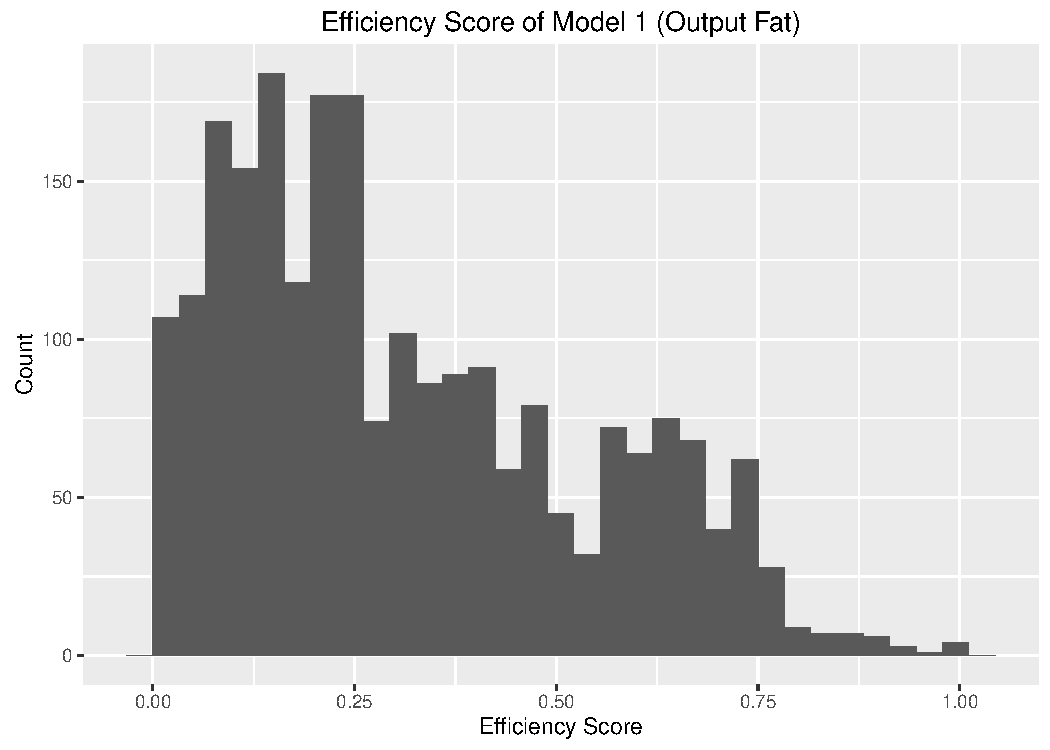
\includegraphics{DEA-DEA_3}
\end{figure}


Figure 2 plots the milk per milk cow production efficiency frontier of farms.

\begin{figure}[h]
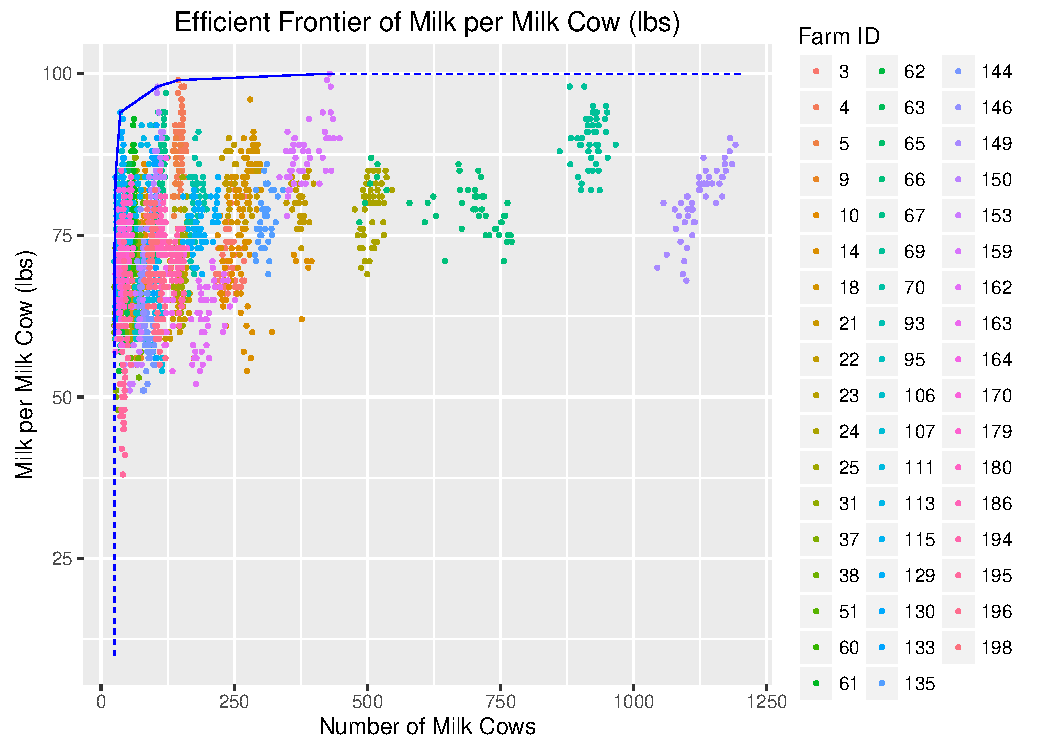
\includegraphics{DEA-Milk_Frontier}
\caption{Efficient Frontier of Milk per Milk Cow (lbs)}
\end{figure}

Figure 3 plots the milk fat production efficiency frontier of farms.

\begin{figure}[h]
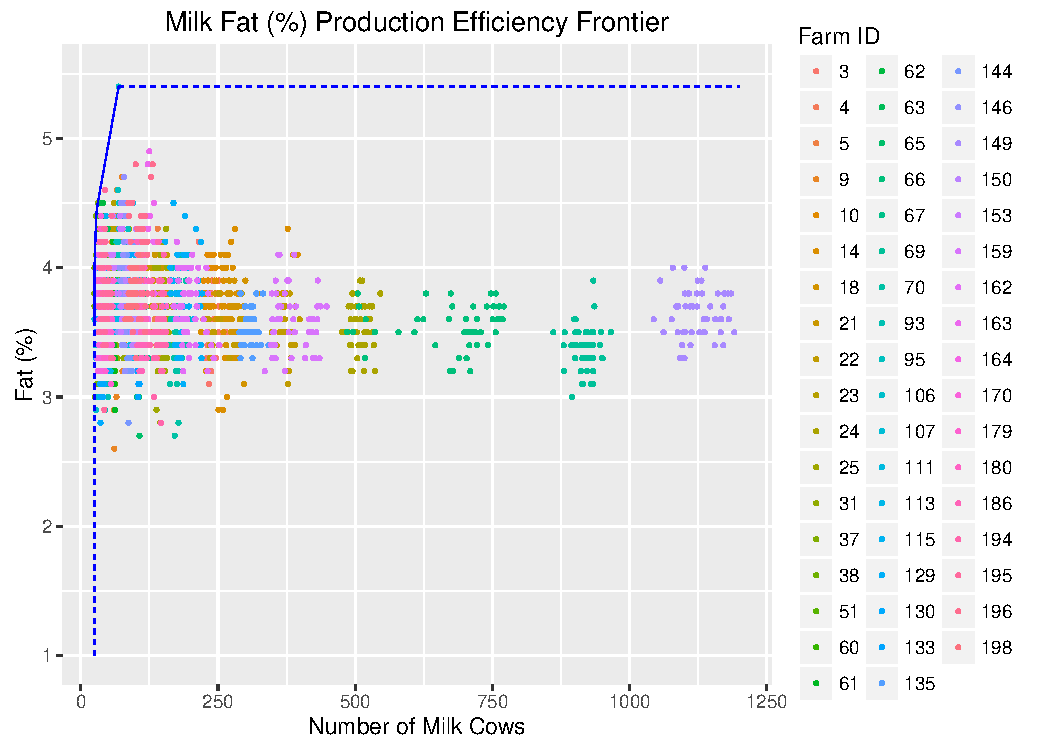
\includegraphics{DEA-Fat_Frontier}
\caption{Milk Fat Production Efficiency Frontier}
\end{figure}

\newpage
Figure 4 plots the milk protein production efficiency frontier of farms.
\begin{figure}[h]
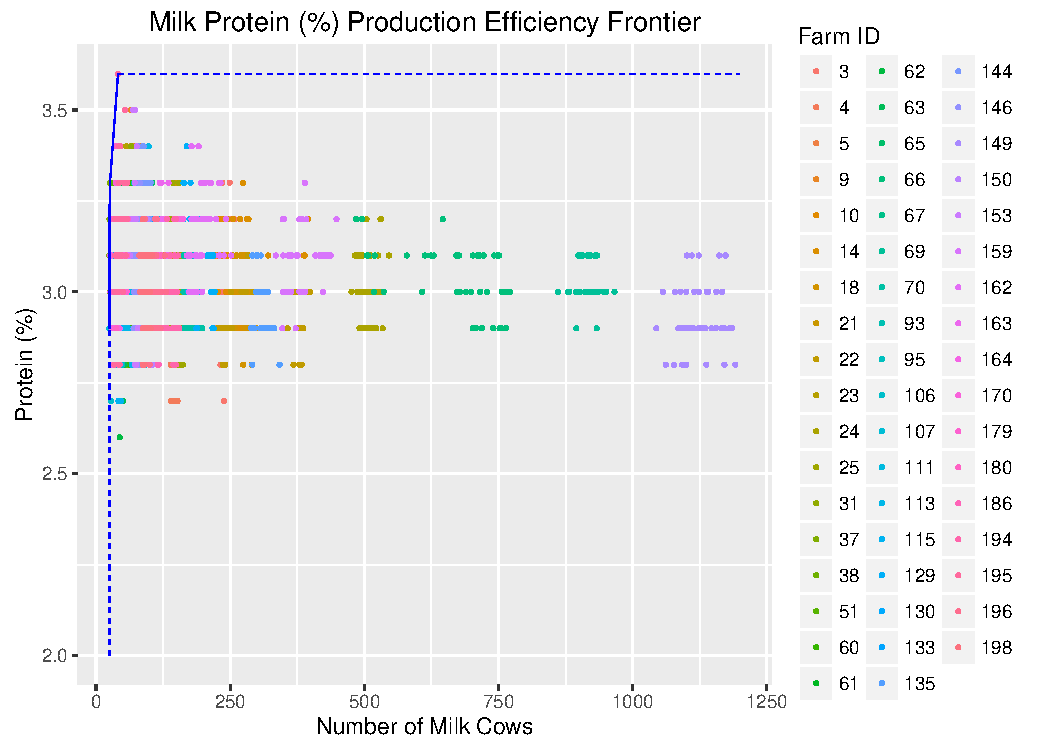
\includegraphics{DEA-Pro_Frontier}
\caption{Milk Protein Production Efficiency Frontier}
\end{figure}




%---------------------------------------------------------------------------------------------------
\newpage
\subsection{Model 2: Multiple Inputs and Outputs DEA on Monthly and Test Data}
%---------------------------------------------------------------------------------------------------
\subsubsection{Model 2-1 DEA of Whole Sample with augmented data}
Next, we add the test data collected. We assume that the test value hold for all months following a test date. Test dates were during Fall and Spring for 2014 and 2015. We specify the production of milk to be a function of the number of milk cows, Dry Matter, CP\%, NDF\% DM, Starch \%DM, Starch Digestibility, NDF Digest, and pH (i.e. inputs of the model). To measure the milk production output, we choose milk (lbs) per milk cow, fat, pro, (negative) MUN and (negative) fecal starch the output vairables. The DEA results can be summarised as follows:


\begin{Schunk}
\begin{Sinput}
> Inputs_model2 = c("X__Milk_Cows", 
+                   "Dry_Matter", 
+                   "CP__", 
+                   "NDF___DM", 
+                   "Starch___DM", 
+                   "pH")
> Outputs_model2_1 = c("Milk_per_Milk_Cow",
+                    "X__Fat",
+                    "X__Pro")
> Outputs_model2_2 = c("Fecal_Starch",
+                      "MUN")
> dea_model2_all = dea(data_good[,Inputs_model2],
+                  cbind(data_good[,Outputs_model2_1], -data_good[,Outputs_model2_2]))
> summary(dea_model2_all)
\end{Sinput}
\begin{Soutput}
Summary of efficiencies
The technology is vrs and input orientated efficiency
Number of firms with efficiency==1 are 891 
Mean efficiency: 0.982 
---                
  Eff range         #  %
  0.9<= E <1     1412 61
        E ==1     891 39
   Min. 1st Qu.  Median    Mean 3rd Qu.    Max. 
 0.9085  0.9689  0.9919  0.9824  1.0000  1.0000 
\end{Soutput}
\end{Schunk}

\subsubsection{Model 2-2 DEA of Whole Sample with original test data}


\begin{Schunk}
\begin{Sinput}
> dea_model2_test = dea(Test_data[,Inputs_model2],
+                       cbind(Test_data[,Outputs_model2_1], -Test_data[,Outputs_model2_2]))
> summary(dea_model2_test)
\end{Sinput}
\begin{Soutput}
Summary of efficiencies
The technology is vrs and input orientated efficiency
Number of firms with efficiency==1 are 104 
Mean efficiency: 0.989 
---                
  Eff range        #  %
  0.9<= E <1      56 35
        E ==1    104 65
   Min. 1st Qu.  Median    Mean 3rd Qu.    Max. 
 0.9034  0.9855  1.0000  0.9893  1.0000  1.0000 
\end{Soutput}
\begin{Sinput}
> summary(dea(Test_data[,Inputs_model2], -Test_data[,Outputs_model2_2[1]]))
\end{Sinput}
\begin{Soutput}
Summary of efficiencies
The technology is vrs and input orientated efficiency
Number of firms with efficiency==1 are 58 
Mean efficiency: 0.977 
---                
  Eff range        #  %
  0.9<= E <1     102 64
        E ==1     58 36
   Min. 1st Qu.  Median    Mean 3rd Qu.    Max. 
 0.9016  0.9616  0.9833  0.9772  1.0000  1.0000 
\end{Soutput}
\begin{Sinput}
> summary(dea(Test_data[,Inputs_model2], -Test_data[,Outputs_model2_2[2]]))
\end{Sinput}
\begin{Soutput}
Summary of efficiencies
The technology is vrs and input orientated efficiency
Number of firms with efficiency==1 are 46 
Mean efficiency: 0.975 
---                
  Eff range        #  %
  0.9<= E <1     114 71
        E ==1     46 29
   Min. 1st Qu.  Median    Mean 3rd Qu.    Max. 
 0.9022  0.9598  0.9775  0.9749  1.0000  1.0000 
\end{Soutput}
\end{Schunk}

%Figure 5 shows the plot of model 2 with 2303 observations.
%\begin{figure}[h]
%<<DEA_21, fig=TRUE, height= 5, width=7, echo=FALSE>>=
%c = ggplot(as.data.frame(dea_model2_all$eff), aes(dea_model2_all$eff))
%c + geom_histogram()  + xlab('Efficiency Score') +
%ylab('Count') +
%ggtitle('Efficiency Score of Model 2 (2303 obs)')
%@
%\caption{Efficiency Score of Model 2 (2303 obs)}
%\end{figure}

Figure 5 shows the plot of model 2 with 160 observations.
\begin{figure}[h]
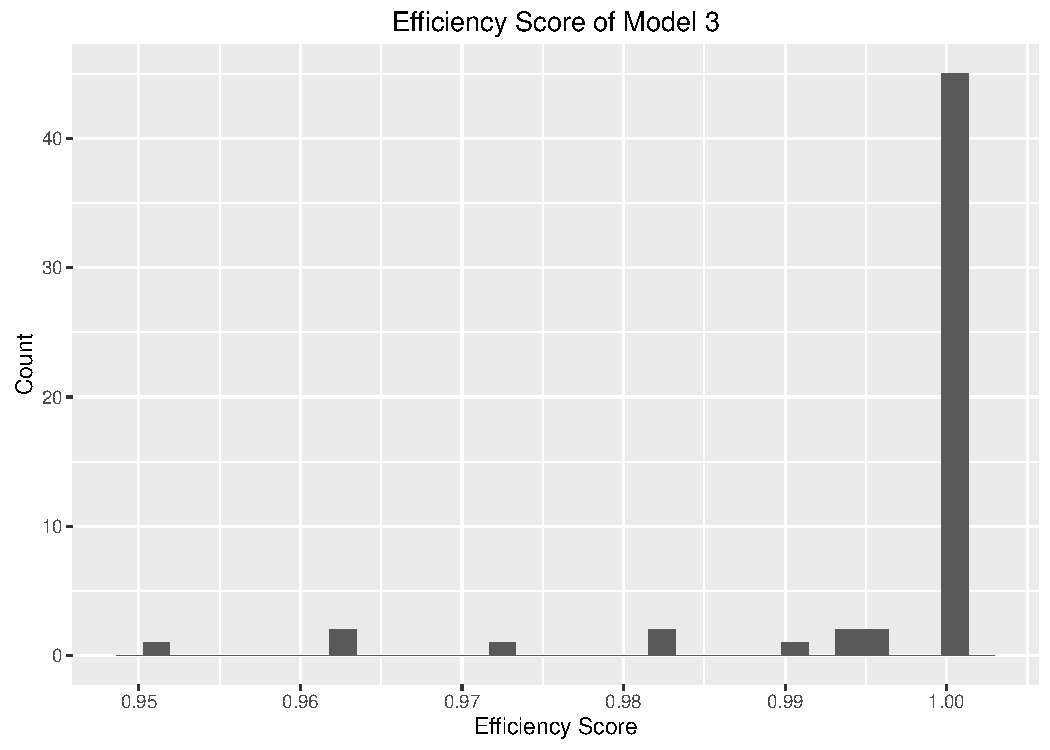
\includegraphics{DEA-DEA_22}
\caption{Efficiency Score of Model 2 (160 obs)}
\end{figure}

Model 2-1 and 2-2 show that with a relatively large number of inputs, all firms have high efficiency score. 


\subsubsection{Model 2-3 DEA of Different Partition of Sample}
From section 1, we conclude there is herterogeneity across different scale of farms. We suspect such herterogeneity will affect the efficiency of DEA analysis. Thus in this section, we partition the whole sample into different subsamples over the number of cows, and do DEA in each subsample. In each subsample, since we have less observations, with consideratin of degree freedom, we only choose some major input variates (Dry matter, CP\%, Starch \%DM, pH). We first plot histrogam of number of cows in the test data.

\begin{figure}[h]
\begin{Schunk}
\begin{Sinput}
> ggplot(Test_data, aes(X__Cows))+
+   geom_histogram()
\end{Sinput}
\end{Schunk}
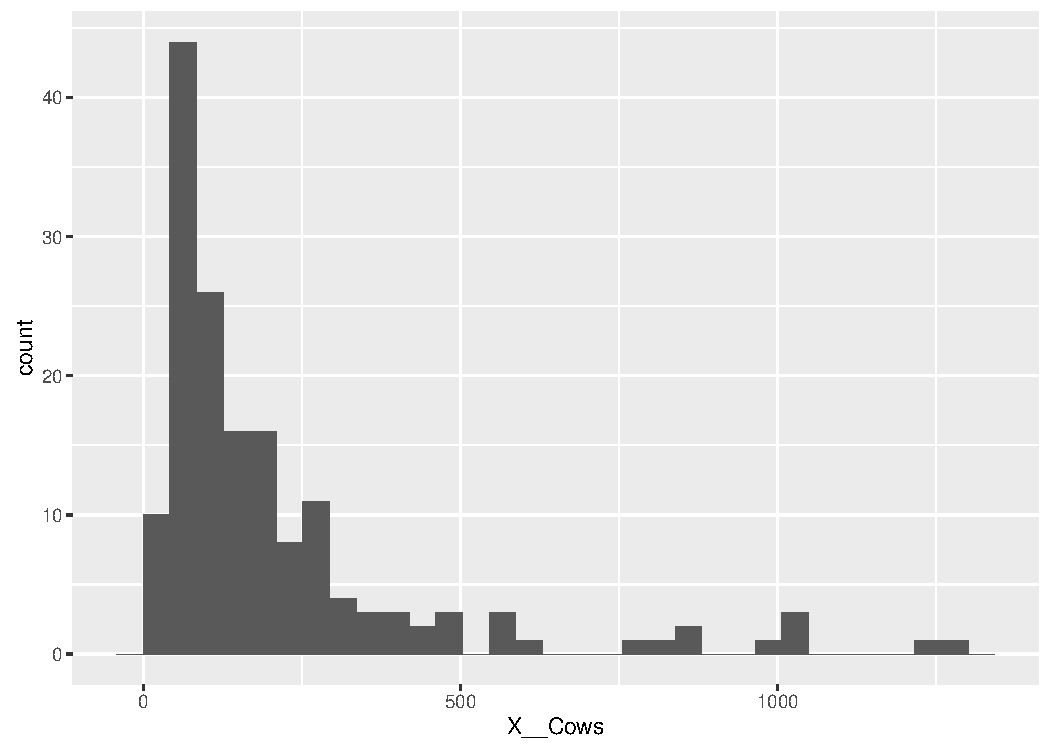
\includegraphics{DEA-Plot1}
\caption{Histogram of number of cows (162 obs)}
\end{figure}

Now we partition data according to number of cows. The thresolds we chose are 100, 275, 400, 550.
\begin{figure}[h]
\begin{Schunk}
\begin{Sinput}
> Test_data1= Test_data
> Test_data1%<>%
+   #group_by(., X__Cows = cut(X__Cows, breaks = c(0, 100, 275, 400, 550, 725, 1000, 2000)))
+     group_by(., X__Cows = cut(X__Cows, breaks = c(0, 100, 275, 400, 550, 2000)))
> ggplot(Test_data1, aes(Dry_Matter, Milk_per_Milk_Cow, color = X__Cows))+
+   geom_point()
\end{Sinput}
\end{Schunk}
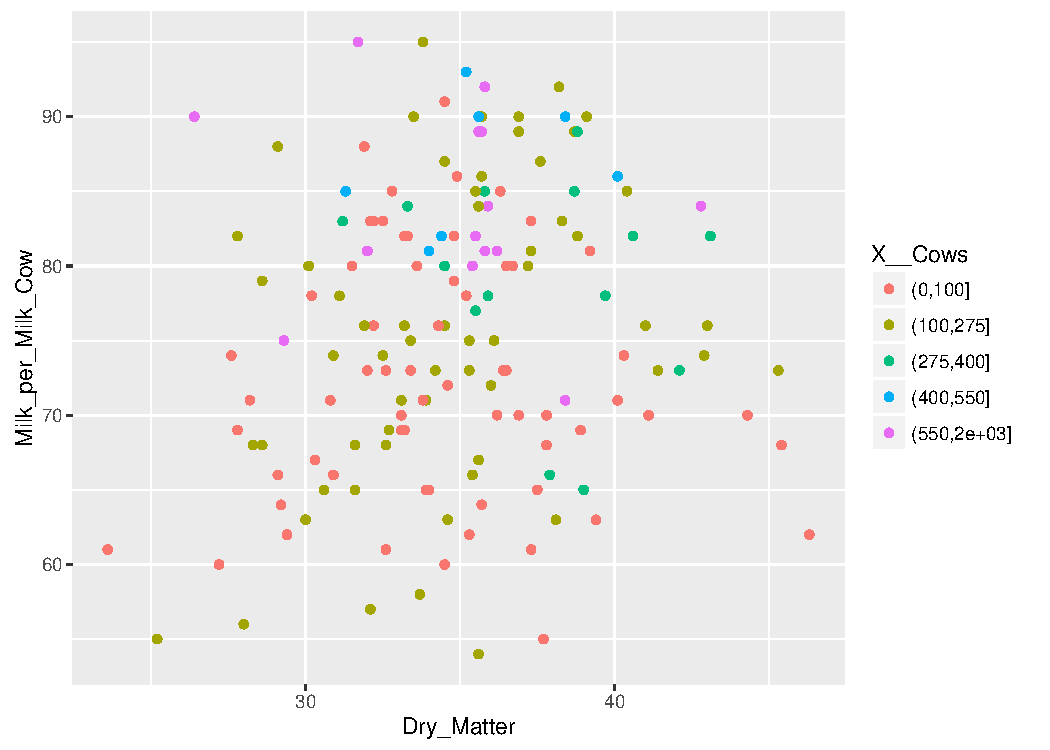
\includegraphics{DEA-partition_data}
\end{figure}


For each subsample, do the DEA. 
\begin{Schunk}
\begin{Sinput}
> try_out = try(
+ Test_data1%>%
+   do({
+    summary(dea(as.data.frame(
+                   select(., Dry_Matter, 
+                   CP__, 
+                   Starch___DM, 
+                   pH)), 
+                as.data.frame(
+                  select(., Milk_per_Milk_Cow,
+                         X__Fat,
+                         X__Fat
+                    ))
+                  ))
+   })
+ )
\end{Sinput}
\begin{Soutput}
Summary of efficiencies
The technology is vrs and input orientated efficiency
Number of firms with efficiency==1 are 17 
Mean efficiency: 0.947 
---                
  Eff range       #  %
  0.8<= E <0.9   11 17
  0.9<= E <1     37 57
        E ==1    17 26
   Min. 1st Qu.  Median    Mean 3rd Qu.    Max. 
 0.8013  0.9160  0.9494  0.9468  1.0000  1.0000 
Summary of efficiencies
The technology is vrs and input orientated efficiency
Number of firms with efficiency==1 are 17 
Mean efficiency: 0.952 
---                
  Eff range       #    %
  0.7<= E <0.8    1  1.7
  0.8<= E <0.9    8 13.3
  0.9<= E <1     34 56.7
        E ==1    17 28.3
   Min. 1st Qu.  Median    Mean 3rd Qu.    Max. 
 0.7676  0.9242  0.9582  0.9520  1.0000  1.0000 
Summary of efficiencies
The technology is vrs and input orientated efficiency
Number of firms with efficiency==1 are 9 
Mean efficiency: 0.988 
---                
  Eff range      #  %
  0.9<= E <1     5 36
        E ==1    9 64
   Min. 1st Qu.  Median    Mean 3rd Qu.    Max. 
 0.9428  0.9816  1.0000  0.9881  1.0000  1.0000 
Summary of efficiencies
The technology is vrs and input orientated efficiency
Number of firms with efficiency==1 are 7 
Mean efficiency: 1 
---                
  Eff range      #   %
        E ==1    7 100
   Min. 1st Qu.  Median    Mean 3rd Qu.    Max. 
      1       1       1       1       1       1 
Summary of efficiencies
The technology is vrs and input orientated efficiency
Number of firms with efficiency==1 are 12 
Mean efficiency: 0.997 
---                
  Eff range       #  %
  0.9<= E <1      2 14
        E ==1    12 86
   Min. 1st Qu.  Median    Mean 3rd Qu.    Max. 
 0.9775  1.0000  1.0000  0.9975  1.0000  1.0000 
\end{Soutput}
\begin{Sinput}
> #cat(try_out)
\end{Sinput}
\end{Schunk}

We plot these result withdry matter as x-axis and milk per milk c ow as y-axis
\begin{figure}[h]
\begin{Schunk}
\begin{Sinput}
> eff_partition = 
+ Test_data1%>%
+   do({
+    data.frame(dea(as.data.frame(
+                   select(., Dry_Matter, 
+                   CP__, 
+                   Starch___DM, 
+                   pH)), 
+                as.data.frame(
+                  select(., Milk_per_Milk_Cow,
+                         X__Fat,
+                         X__Fat
+                    ))
+                  )$eff)
+   })
> colnames(eff_partition)[2] = "Efficiency"
> ggplot(eff_partition, aes(Efficiency, fill = X__Cows))+
+   geom_histogram(position = "stack")
\end{Sinput}
\end{Schunk}
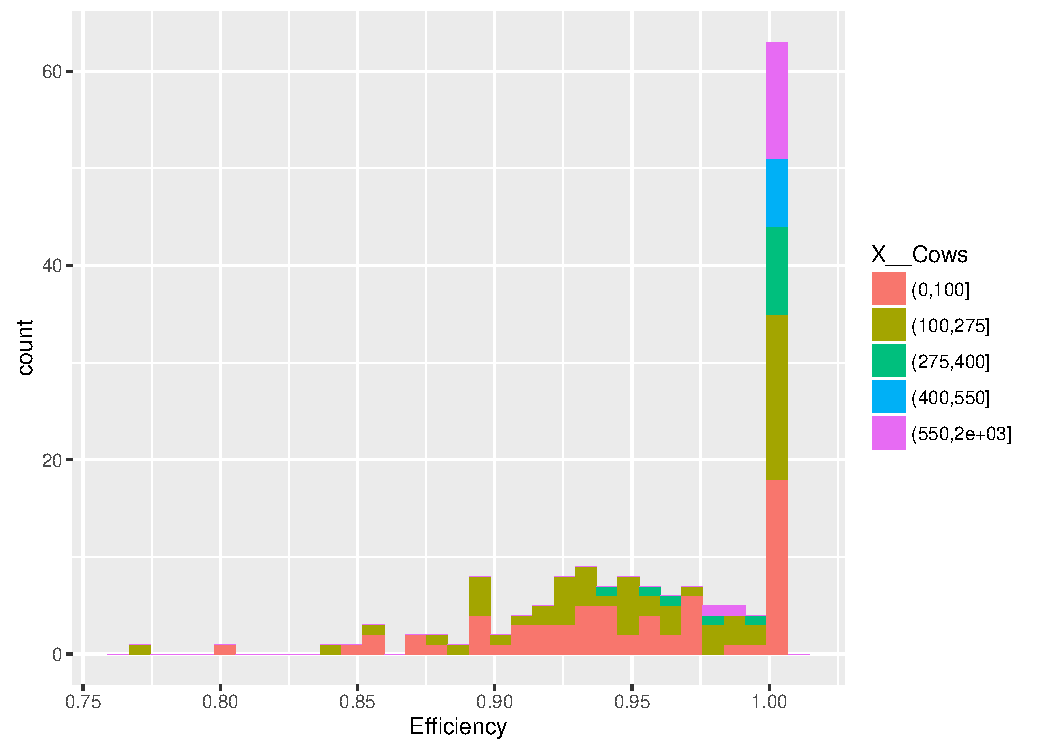
\includegraphics{DEA-Plot_Model_23}
\caption{Histogram of Efficiency by Group}
\end{figure}

%-----------------------------------------------------------------
\subsection{Model 3: DEA with Aggregation of Annual Data}
%-----------------------------------------------------------------
To integrate the year data of these farms, we merge the monthly data and annual data by Farm ID and year.
\begin{Schunk}
\begin{Sinput}
> data_year = read.xlsx(file = "Annual.xlsx", 3)
> data_year$Farm_ID = factor(data_year$Farm_ID)
> data_new = merge(data, data_year, by = c("Farm_ID", "year"),
+                  all.x = T)
> dim(data_new)
\end{Sinput}
\begin{Soutput}
[1] 2303   60
\end{Soutput}
\end{Schunk}
We see we added in 34 variates. To check we are not losing any observations, we have
\begin{Schunk}
\begin{Sinput}
> sum(data_new$Farm_ID == data$Farm_ID)
\end{Sinput}
\begin{Soutput}
[1] 2303
\end{Soutput}
\end{Schunk}
Thus we did not lose any observation. To check the number of missing values in each variate, we have

\begin{Schunk}
\begin{Sinput}
> result = sapply(1:dim(data_new)[2], function(x) missing_fn(x))
> missing_value_new = as.data.frame(result)
> missing_value_new$Var = colnames(data_new)
> colnames(missing_value_new)[1] = "Number_of_Missing_Values"
> missing_value_new = missing_value_new[, c(2, 1)]
> missing_tab1 = xtable(missing_value_new, 
+                     caption = "Number of Missing Values (Annual)",
+                     label = "Table-5")
> print(missing_tab1, latex.environments = "center", size = "small", 
+       tabular.environment = "longtable")
\end{Sinput}
% latex table generated in R 3.2.2 by xtable 1.8-2 package
% Thu Mar 31 14:30:18 2016
\begingroup\small
\begin{longtable}{rlr}
  \hline
 & Var & Number\_of\_Missing\_Values \\ 
  \hline
1 & Farm\_ID &   0 \\ 
  2 & year &   0 \\ 
  3 & Herdcode &   0 \\ 
  4 & Milk\_per\_Milk\_Cow &   0 \\ 
  5 & X\_\_Fat &   0 \\ 
  6 & X\_\_Pro &   0 \\ 
  7 & X\_\_Cows &   0 \\ 
  8 & ME\_305\_Milk &  11 \\ 
  9 & ME\_305\_Fat &  11 \\ 
  10 & ME\_305\_Pro &  11 \\ 
  11 & X\_\_Milk\_Cows &   0 \\ 
  12 & X\_50\_D\_Milk &   0 \\ 
  13 & Peak &  11 \\ 
  14 & Summit &  11 \\ 
  15 & DHIDate &   0 \\ 
  16 & month &   0 \\ 
  17 & Sample\_Number & 2143 \\ 
  18 & Season\_Year & 2143 \\ 
  19 & MUN & 2144 \\ 
  20 & Dry\_Matter & 2143 \\ 
  21 & CP\_\_ & 2143 \\ 
  22 & NDF\_\_\_DM & 2143 \\ 
  23 & Starch\_\_\_DM & 2143 \\ 
  24 & Starch\_Digestibility & 2143 \\ 
  25 & NDF\_Digestibility & 2178 \\ 
  26 & NDF\_Dig\_Group & 2189 \\ 
  27 & Fecal\_Starch & 2143 \\ 
  28 & pH & 2158 \\ 
  29 & Hybrid & 2215 \\ 
  30 & Structure & 2215 \\ 
  31 & SampleDate & 2143 \\ 
  32 & Parent\_Company & 2249 \\ 
  33 & Hybrid\_Company & 2247 \\ 
  34 & Hybrid\_Name & 2249 \\ 
  35 & Trait & 2258 \\ 
  36 & relative\_maturity & 2249 \\ 
  37 & CWT\_Sold & 1391 \\ 
  38 & Dairy\_IOFC\_Surplus\_Group & 1391 \\ 
  39 & Crop\_Cost\_Calc & 1391 \\ 
  40 & Pur\_Feed\_Calc & 1391 \\ 
  41 & Feed\_Cost\_\_All\_Animals\_\_Annual & 1391 \\ 
  42 & Kernel\_Processed & 2303 \\ 
  43 & Inoculant\_Applied\_ & 2303 \\ 
  44 & Inoculent\_1 & 2303 \\ 
  45 & Inoculent\_Original & 2303 \\ 
  46 & Inoculent\_2 & 2303 \\ 
  47 & Dry\_Matter\_Eval & 2303 \\ 
  48 & Particle\_Size\_Eval & 2303 \\ 
  49 & BMP2a & 2303 \\ 
  50 & BMP2B & 2303 \\ 
  51 & BMP2C & 2303 \\ 
  52 & BMP2D & 2303 \\ 
  53 & BMP3 & 2303 \\ 
  54 & BMP4 & 2303 \\ 
  55 & newyear & 2303 \\ 
  56 & Corn\_silage & 1946 \\ 
  57 & Alfalfa\_sil & 2108 \\ 
  58 & Alfalfa\_hay & 2244 \\ 
  59 & Grass\_Silage & 2252 \\ 
  60 & Small\_Grain\_Sil & 2109 \\ 
   \hline
\hline
\caption{Number of Missing Values (Annual)} 
\label{Table-5}
\end{longtable}
\endgroup\end{Schunk}


\subsubsection{Model 3-1 Annual Data Variables as Inputs}

To analyze production efficiency, we would like to use purchased feed, corn silage, crop cost and number of milk cows as inputs, and milk (lbs) per milk cow as output. We see there are some missing values in the input variates. In this case, we only use those oberservations with no missing values (otherwise, the efficiency score goes to infinity).
\begin{Schunk}
\begin{Sinput}
> data_new_no_missing = data_new[!(is.na(data_new$Pur_Feed_Calc) |
+                                 is.na(data_new$Corn_silage) |
+                                 is.na(data_new$Crop_Cost_Calc)), ] 
> 
\end{Sinput}
\end{Schunk}
Now we do DEA using this new data with no missing values.
\begin{Schunk}
\begin{Sinput}
> dea_four_input = dea(cbind(data_new_no_missing$X__Milk_Cows, 
+                            data_new_no_missing$Pur_Feed_Calc,
+                            data_new_no_missing$Corn_silage, 
+                            data_new_no_missing$Crop_Cost_Calc), 
+                      matrix(data_new_no_missing$Milk_per_Milk_Cow))
> summary(dea_four_input)
\end{Sinput}
\begin{Soutput}
Summary of efficiencies
The technology is vrs and input orientated efficiency
Number of firms with efficiency==1 are 114 
Mean efficiency: 0.895 
---                
  Eff range        #    %
  0.6<= E <0.7    20  5.6
  0.7<= E <0.8    63 17.6
  0.8<= E <0.9    48 13.4
  0.9<= E <1     112 31.4
        E ==1    114 31.9
   Min. 1st Qu.  Median    Mean 3rd Qu.    Max. 
 0.6222  0.8048  0.9272  0.8947  1.0000  1.0000 
\end{Soutput}
\end{Schunk}
We see there 114 observations with production efficiency 1. For visualization, since there are four inputs and one output, we aggregate the inputs as X by summation (same as the R function \textit{dea.plot} does)\footnote{This is only for visualization purpose.}. Figure 5 shows the result. Observation with efficiency 1 (on the production efficiency frontier) are marked by crossmarks.

\begin{figure}[h]
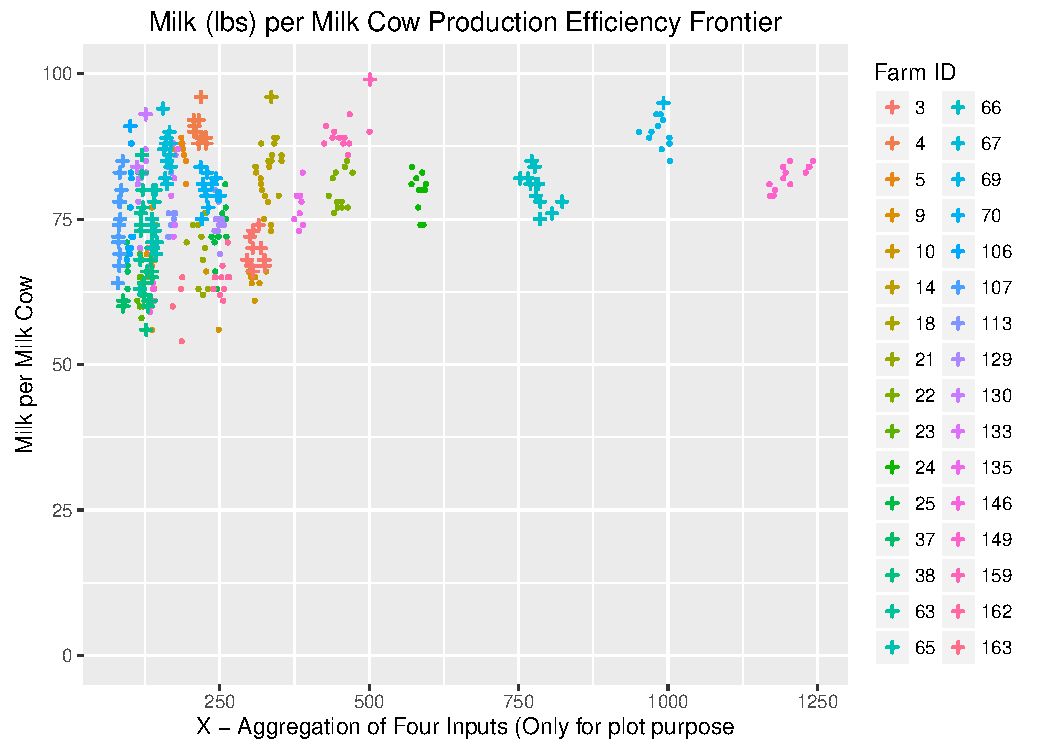
\includegraphics{DEA-Four_Input_DEA}
\caption{Milk per Milk Cow Production Efficiency Frontier}
\end{figure}


We also conducted DEA of multiple inputs and multiple outputs model. Inputs are the number of milk cows, Dry Matter, CP\%, NDF\% DM, Starch \%DM, Starch Digestibility, NDF Digest, pH (i.e. inputs of the model), Dairy IOFC Surplus Group, Crop Cost, Pur Feed, Feed Cost, and Corn silage. The output variates are milk (lbs) per milk cow, fat, pro, (negative) MUN and (negative) fecal starch. The DEA results can be summarised as follows:
\begin{Schunk}
\begin{Sinput}
> Inputs_model3 = c(Inputs_model2,
+                   "Dairy_IOFC_Surplus_Group",
+                   "Crop_Cost_Calc",
+                   "Pur_Feed_Calc",
+                   "Feed_Cost__All_Animals__Annual",
+                   "Corn_silage"
+                   )
\end{Sinput}
\end{Schunk}

\begin{Schunk}
\begin{Soutput}
Summary of efficiencies
The technology is vrs and input orientated efficiency
Number of firms with efficiency==1 are 45 
Mean efficiency: 0.996 
---                
  Eff range       #  %
  0.9<= E <1     11 20
        E ==1    45 80
   Min. 1st Qu.  Median    Mean 3rd Qu.    Max. 
 0.9506  1.0000  1.0000  0.9961  1.0000  1.0000 
\end{Soutput}
\end{Schunk}


\begin{figure}[h]
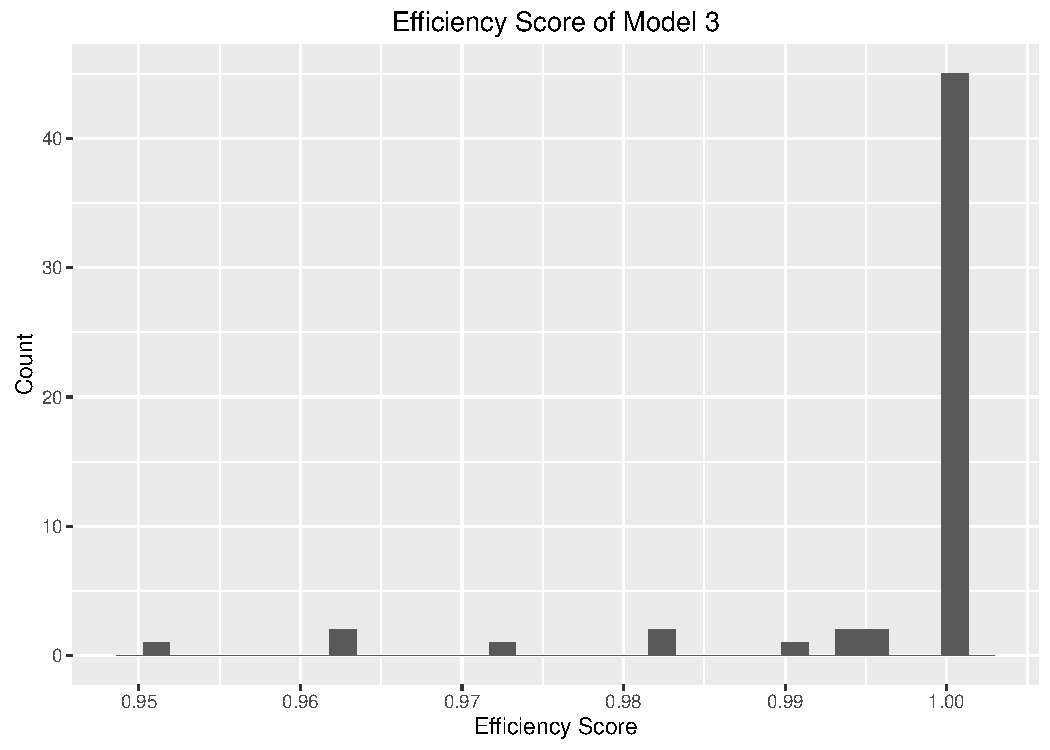
\includegraphics{DEA-DEA_22}
\end{figure}

The result resemables that of model 2. Every observation has a high efficiency score. This says in the DEA with (relatively) large number of input, almost every firm is efficient.


\subsubsection{Model 3-2 Two-Step DEA on the Whole Annual Data}
\textbf{Step 1}: For the whole data, we estimate efficiency score using DEA.
\begin{Schunk}
\begin{Sinput}
> Inputs_model32 = c("X__Milk_Cows", 
+                   "Dry_Matter", 
+                   "CP__", 
+                   "Starch___DM", 
+                   "pH")
> Outputs_model32 = c("Milk_per_Milk_Cow",
+                    "X__Fat",
+                    "X__Pro")
> dea321 = dea(data_model3[,Inputs_model32],
+                  data_model3[,Outputs_model32[1]])
> summary(dea321)
\end{Sinput}
\begin{Soutput}
Summary of efficiencies
The technology is vrs and input orientated efficiency
Number of firms with efficiency==1 are 25 
Mean efficiency: 0.972 
---                
  Eff range       #    %
  0.8<= E <0.9    2  3.6
  0.9<= E <1     29 51.8
        E ==1    25 44.6
   Min. 1st Qu.  Median    Mean 3rd Qu.    Max. 
 0.8909  0.9507  0.9864  0.9723  1.0000  1.0000 
\end{Soutput}
\begin{Sinput}
> dea322 = dea(data_model3[,Inputs_model32],
+                  data_model3[,Outputs_model32[2]])
> summary(dea322)
\end{Sinput}
\begin{Soutput}
Summary of efficiencies
The technology is vrs and input orientated efficiency
Number of firms with efficiency==1 are 12 
Mean efficiency: 0.955 
---                
  Eff range       #    %
  0.8<= E <0.9    4  7.1
  0.9<= E <1     40 71.4
        E ==1    12 21.4
   Min. 1st Qu.  Median    Mean 3rd Qu.    Max. 
 0.8814  0.9332  0.9509  0.9553  0.9911  1.0000 
\end{Soutput}
\begin{Sinput}
> dea323 = dea(data_model3[,Inputs_model32],
+                  data_model3[,Outputs_model32[3]])
> summary(dea323)
\end{Sinput}
\begin{Soutput}
Summary of efficiencies
The technology is vrs and input orientated efficiency
Number of firms with efficiency==1 are 16 
Mean efficiency: 0.959 
---                
  Eff range       #    %
  0.8<= E <0.9    4  7.1
  0.9<= E <1     36 64.3
        E ==1    16 28.6
   Min. 1st Qu.  Median    Mean 3rd Qu.    Max. 
 0.8814  0.9378  0.9565  0.9590  1.0000  1.0000 
\end{Soutput}
\end{Schunk}

\textbf{Step 2}: We run a tobit regression of efficiency score on four annual variates (daily IOFC Surplus Group, Crop Cost, Purchased Feed and Corn Silage). The results are as follows.
\begin{Schunk}
\begin{Sinput}
> tobit_1 = censReg(dea321$eff~data_model3$Dairy_IOFC_Surplus_Group +
+                   data_model3$Crop_Cost_Calc+
+                   data_model3$Pur_Feed_Calc+
+                   #data_model3$Feed_Cost__All_Animals__Annual+
+                   data_model3$Corn_silage, right = 1)
> summary(tobit_1)
\end{Sinput}
\begin{Soutput}
Call:
censReg(formula = dea321$eff ~ data_model3$Dairy_IOFC_Surplus_Group + 
    data_model3$Crop_Cost_Calc + data_model3$Pur_Feed_Calc + 
    data_model3$Corn_silage, right = 1)

Observations:
         Total  Left-censored     Uncensored Right-censored 
            56              0             31             25 

Coefficients:
                                       Estimate Std. error t value Pr(> t)    
(Intercept)                           0.8774553  0.0617451  14.211  <2e-16 ***
data_model3$Dairy_IOFC_Surplus_Group  0.0005233  0.0005318   0.984   0.325    
data_model3$Crop_Cost_Calc           -0.0031480  0.0067828  -0.464   0.643    
data_model3$Pur_Feed_Calc             0.0058907  0.0045398   1.298   0.194    
data_model3$Corn_silage               0.0010717  0.0006683   1.604   0.109    
logSigma                             -3.0056183  0.1412398 -21.280  <2e-16 ***
---
Signif. codes:  0 '***' 0.001 '**' 0.01 '*' 0.05 '.' 0.1 ' ' 1

Newton-Raphson maximisation, 12 iterations
Return code 2: successive function values within tolerance limit
Log-likelihood: 30.53812 on 6 Df
\end{Soutput}
\begin{Sinput}
> tobit_1 = censReg(dea322$eff~data_model3$Dairy_IOFC_Surplus_Group +
+                   data_model3$Crop_Cost_Calc+
+                   data_model3$Pur_Feed_Calc+
+                   #data_model3$Feed_Cost__All_Animals__Annual+
+                   data_model3$Corn_silage, right = 1)
> summary(tobit_1)
\end{Sinput}
\begin{Soutput}
Call:
censReg(formula = dea322$eff ~ data_model3$Dairy_IOFC_Surplus_Group + 
    data_model3$Crop_Cost_Calc + data_model3$Pur_Feed_Calc + 
    data_model3$Corn_silage, right = 1)

Observations:
         Total  Left-censored     Uncensored Right-censored 
            56              0             44             12 

Coefficients:
                                       Estimate Std. error t value Pr(> t)    
(Intercept)                           9.256e-01  4.776e-02  19.378  <2e-16 ***
data_model3$Dairy_IOFC_Surplus_Group -1.788e-04  4.033e-04  -0.444   0.657    
data_model3$Crop_Cost_Calc            6.287e-03  5.461e-03   1.151   0.250    
data_model3$Pur_Feed_Calc             2.794e-03  3.406e-03   0.820   0.412    
data_model3$Corn_silage              -1.032e-05  5.238e-04  -0.020   0.984    
logSigma                             -3.195e+00  1.130e-01 -28.270  <2e-16 ***
---
Signif. codes:  0 '***' 0.001 '**' 0.01 '*' 0.05 '.' 0.1 ' ' 1

Newton-Raphson maximisation, 11 iterations
Return code 2: successive function values within tolerance limit
Log-likelihood: 65.52005 on 6 Df
\end{Soutput}
\begin{Sinput}
> tobit_1 = censReg(dea323$eff~data_model3$Dairy_IOFC_Surplus_Group +
+                   data_model3$Crop_Cost_Calc+
+                   data_model3$Pur_Feed_Calc+
+                   #data_model3$Feed_Cost__All_Animals__Annual+
+                   data_model3$Corn_silage, right = 1)
> summary(tobit_1)
\end{Sinput}
\begin{Soutput}
Call:
censReg(formula = dea323$eff ~ data_model3$Dairy_IOFC_Surplus_Group + 
    data_model3$Crop_Cost_Calc + data_model3$Pur_Feed_Calc + 
    data_model3$Corn_silage, right = 1)

Observations:
         Total  Left-censored     Uncensored Right-censored 
            56              0             40             16 

Coefficients:
                                       Estimate Std. error t value Pr(> t)    
(Intercept)                           9.079e-01  5.251e-02  17.291  <2e-16 ***
data_model3$Dairy_IOFC_Surplus_Group -9.149e-06  4.356e-04  -0.021  0.9832    
data_model3$Crop_Cost_Calc            1.232e-02  6.090e-03   2.023  0.0431 *  
data_model3$Pur_Feed_Calc             1.848e-03  3.676e-03   0.503  0.6152    
data_model3$Corn_silage               1.599e-04  5.747e-04   0.278  0.7808    
logSigma                             -3.127e+00  1.206e-01 -25.924  <2e-16 ***
---
Signif. codes:  0 '***' 0.001 '**' 0.01 '*' 0.05 '.' 0.1 ' ' 1

Newton-Raphson maximisation, 12 iterations
Return code 1: gradient close to zero
Log-likelihood: 53.24037 on 6 Df
\end{Soutput}
\begin{Sinput}
> 
\end{Sinput}
\end{Schunk}


\subsubsection{Model 3-3 Two-Step DEA on partitioned Annual Data}

\textbf{Step 1}: For each group, we estimate efficiency score using DEA. The results are as follows.
\begin{Schunk}
\begin{Sinput}
> data_model3_1 =data_model3
> data_model3_1%<>%
+   #group_by(., X__Cows = cut(X__Cows, breaks = c(0, 100, 275, 400, 550, 725, 1000, 2000)))
+     group_by(., X__Cows = cut(X__Cows, breaks = c(0, 100, 275, 450, 2000)))
> try(data_model3_1%>%
+   do({
+    summary(dea(as.data.frame(
+                   select(., Dry_Matter, 
+                   CP__, 
+                   Starch___DM, 
+                   pH)), 
+                as.data.frame(
+                  select(., Milk_per_Milk_Cow,
+                         X__Fat,
+                         X__Fat
+                    ))
+                  ))
+   }))
\end{Sinput}
\begin{Soutput}
Summary of efficiencies
The technology is vrs and input orientated efficiency
Number of firms with efficiency==1 are 9 
Mean efficiency: 0.976 
---                
  Eff range      #    %
  0.8<= E <0.9   1  5.3
  0.9<= E <1     9 47.4
        E ==1    9 47.4
   Min. 1st Qu.  Median    Mean 3rd Qu.    Max. 
 0.8824  0.9605  0.9858  0.9763  1.0000  1.0000 
Summary of efficiencies
The technology is vrs and input orientated efficiency
Number of firms with efficiency==1 are 12 
Mean efficiency: 0.981 
---                
  Eff range       #  %
  0.8<= E <0.9    1  5
  0.9<= E <1      7 35
        E ==1    12 60
   Min. 1st Qu.  Median    Mean 3rd Qu.    Max. 
 0.8911  0.9695  1.0000  0.9811  1.0000  1.0000 
Summary of efficiencies
The technology is vrs and input orientated efficiency
Number of firms with efficiency==1 are 6 
Mean efficiency: 0.988 
---                
  Eff range      #  %
  0.9<= E <1     2 25
        E ==1    6 75
   Min. 1st Qu.  Median    Mean 3rd Qu.    Max. 
 0.9200  0.9964  1.0000  0.9882  1.0000  1.0000 
Summary of efficiencies
The technology is vrs and input orientated efficiency
Number of firms with efficiency==1 are 8 
Mean efficiency: 0.997 
---                
  Eff range      #  %
  0.9<= E <1     1 11
        E ==1    8 89
   Min. 1st Qu.  Median    Mean 3rd Qu.    Max. 
 0.9766  1.0000  1.0000  0.9974  1.0000  1.0000 
\end{Soutput}
\end{Schunk}

Then we attach efficiency scores to the data (by group) and plot them.
\begin{Schunk}
\begin{Sinput}
> data_model3_1%<>% 
+ do({eff =
+ data.frame(
+   dea(as.data.frame(
+                   select(., Dry_Matter, 
+                   CP__, 
+                   Starch___DM, 
+                   pH)), 
+                as.data.frame(
+                  select(., Milk_per_Milk_Cow,
+                         X__Fat,
+                         X__Fat
+                    ))
+                  )$eff
+   )
+ bind_cols(.,eff)})%>%
+ rename(eff = dea.as.data.frame.select....Dry_Matter..CP__..Starch___DM..pH....)
\end{Sinput}
\end{Schunk}


\begin{figure}[h]
\begin{Schunk}
\begin{Sinput}
> eff_partition33= 
+ data_model3_1%>%
+   do({
+    data.frame(dea(as.data.frame(
+                   select(., Dry_Matter, 
+                   CP__, 
+                   Starch___DM, 
+                   pH)), 
+                as.data.frame(
+                  select(., Milk_per_Milk_Cow
+ #                        X__Fat,
+ #                        X__Fat
+                    ))
+                  )$eff)
+   })
> colnames(eff_partition33)[2] = "Efficiency"
> ggplot(eff_partition33, aes(Efficiency, fill = X__Cows))+
+   geom_histogram(position = "stack")
\end{Sinput}
\end{Schunk}
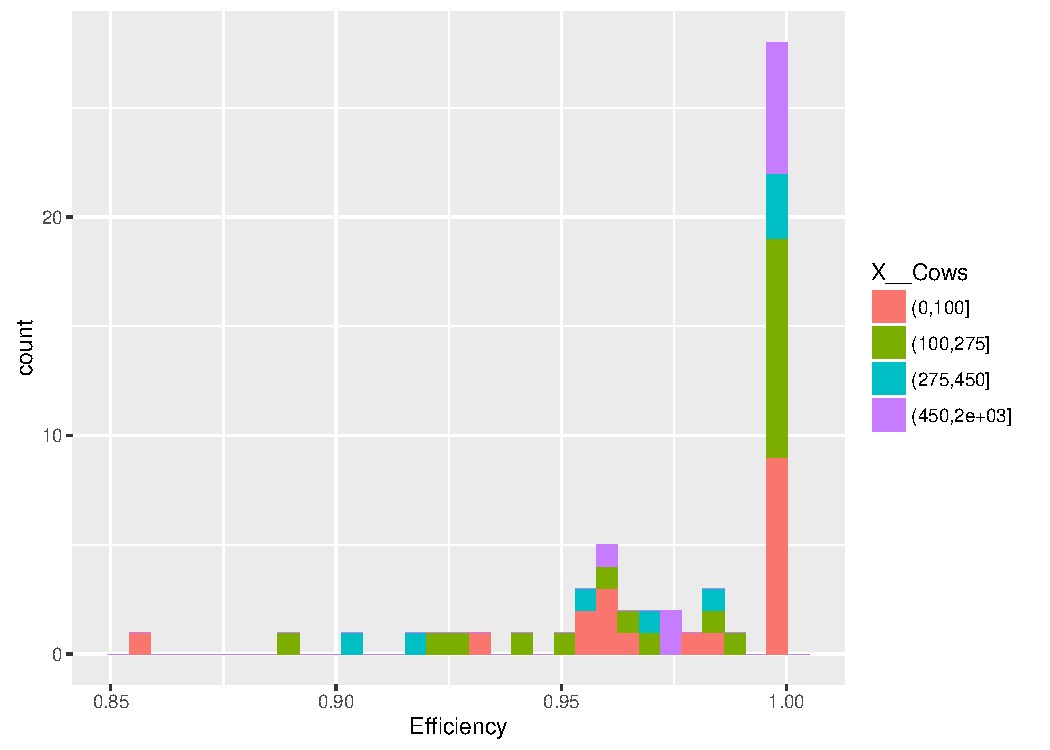
\includegraphics{DEA-Plot_Model_33}
\caption{Histogram of Efficiency of Partitioned Annual Data by Group}
\end{figure}

\textbf{Step 2}: For each group, we run a tobit regression of efficiency score on four annual variates (daily IOFC Surplus Group, Crop Cost, Purchased Feed and Corn Silage). The results are as follows.
%<<>>=
%try(data_model3_1%>%
%  do({tobit = censReg(eff~Dairy_IOFC_Surplus_Group +
%                  Crop_Cost_Calc+
%                  Pur_Feed_Calc+
%                  #Feed_Cost__All_Animals__Annual+
%                  Corn_silage, data = .)
%    summary(tobit)
%    })
%
%)
\begin{Schunk}
\begin{Sinput}
> data_model3_1%<>%
+   mutate(index = as.numeric(X__Cows))
> for (i in 1:4){
+   local_data = 
+     data_model3_1%>%  
+     filter(index == i)
+   
+     local_tobit = censReg(eff~Dairy_IOFC_Surplus_Group +
+                   Crop_Cost_Calc+
+                   Pur_Feed_Calc+
+                   Corn_silage, data = local_data, right =  1)
+     cat("These are the results for the group", as.character(i))
+     print(summary(local_tobit))
+   }
\end{Sinput}
\begin{Soutput}
These are the results for the group 1
Call:
censReg(formula = eff ~ Dairy_IOFC_Surplus_Group + Crop_Cost_Calc + 
    Pur_Feed_Calc + Corn_silage, right = 1, data = local_data)

Observations:
         Total  Left-censored     Uncensored Right-censored 
            19              0             10              9 

Coefficients:
                          Estimate Std. error t value Pr(> t)    
(Intercept)               0.787203   0.179052   4.397 1.1e-05 ***
Dairy_IOFC_Surplus_Group  0.001128   0.001335   0.845   0.398    
Crop_Cost_Calc            0.002178   0.011910   0.183   0.855    
Pur_Feed_Calc             0.001464   0.007281   0.201   0.841    
Corn_silage               0.002869   0.001917   1.497   0.134    
logSigma                 -3.094505   0.249960 -12.380 < 2e-16 ***
---
Signif. codes:  0 '***' 0.001 '**' 0.01 '*' 0.05 '.' 0.1 ' ' 1

Newton-Raphson maximisation, 13 iterations
Return code 1: gradient close to zero
Log-likelihood: 10.35414 on 6 Df

These are the results for the group 2
Call:
censReg(formula = eff ~ Dairy_IOFC_Surplus_Group + Crop_Cost_Calc + 
    Pur_Feed_Calc + Corn_silage, right = 1, data = local_data)

Observations:
         Total  Left-censored     Uncensored Right-censored 
            20              0              8             12 

Coefficients:
                          Estimate Std. error t value Pr(> t)    
(Intercept)               0.933654   0.089970  10.377 < 2e-16 ***
Dairy_IOFC_Surplus_Group  0.001554   0.001135   1.369 0.17102    
Crop_Cost_Calc           -0.026642   0.013184  -2.021 0.04331 *  
Pur_Feed_Calc            -0.004005   0.008739  -0.458 0.64672    
Corn_silage               0.002687   0.000938   2.864 0.00418 ** 
logSigma                 -3.172542   0.281965 -11.252 < 2e-16 ***
---
Signif. codes:  0 '***' 0.001 '**' 0.01 '*' 0.05 '.' 0.1 ' ' 1

Newton-Raphson maximisation, 14 iterations
Return code 1: gradient close to zero
Log-likelihood: 8.012397 on 6 Df

These are the results for the group 3
Call:
censReg(formula = eff ~ Dairy_IOFC_Surplus_Group + Crop_Cost_Calc + 
    Pur_Feed_Calc + Corn_silage, right = 1, data = local_data)

Observations:
         Total  Left-censored     Uncensored Right-censored 
             8              0              2              6 

Coefficients:
                          Estimate Std. error t value Pr(> t)
(Intercept)               1.414183        Inf       0       1
Dairy_IOFC_Surplus_Group  0.003349        Inf       0       1
Crop_Cost_Calc           -0.018938        Inf       0       1
Pur_Feed_Calc             0.008209        Inf       0       1
Corn_silage              -0.007911        Inf       0       1
logSigma                 -4.774835        Inf       0       1

Newton-Raphson maximisation, 17 iterations
Return code 2: successive function values within tolerance limit
Log-likelihood: 5.805917 on 6 Df

These are the results for the group 4
Call:
censReg(formula = eff ~ Dairy_IOFC_Surplus_Group + Crop_Cost_Calc + 
    Pur_Feed_Calc + Corn_silage, right = 1, data = local_data)

Observations:
         Total  Left-censored     Uncensored Right-censored 
             9              0              1              8 

Coefficients:
                           Estimate Std. error t value Pr(> t)
(Intercept)               1.198e+00        Inf       0       1
Dairy_IOFC_Surplus_Group  4.158e-04        Inf       0       1
Crop_Cost_Calc            9.519e-03        Inf       0       1
Pur_Feed_Calc             2.365e-02        Inf       0       1
Corn_silage              -7.002e-03        Inf       0       1
logSigma                 -7.322e+01        Inf       0       1

Newton-Raphson maximisation, 1 iterations
Return code 3: Last step could not find a value above the current.
Boundary of parameter space?  
Consider switching to a more robust optimisation method temporarily.
Log-likelihood: -2.446026e+31 on 6 Df
\end{Soutput}
\begin{Sinput}
> 
\end{Sinput}
\end{Schunk}

%%%%%%%%%%%%%%%%%%%%%%%%%%%%%%%%%%%%
%\newpage
%\section{Appendix}
%\subsection{Detailed Efficiency Scores in Section 3 (One Input)}
%
%<<results= tex>>=
%eff_tab = xtable(eff,
%                caption = "Detailed Efficiency 
%                Scores in Section 3 (One Input)", 
%                label = "Table-6")
%print(eff_tab, latex.environments = "center", size =  "small", 
%     tabular.environment = "longtable")
%@
%
%\subsection{Detailed Efficiency Scores in Section 4 (Four Inputs)}
%<<results= tex>>=
%M = as.data.frame(dea_four_input$eff)
%M$Farm_ID = data_new_no_missing$Farm_ID
%M = M[,c(2, 1)]
%eff_tab_four = xtable(M,
%                caption = "Detailed Efficiency 
%                Scores in Section 4 (Four Inputs)", 
%                label = "Table-7")
%print(eff_tab_four, latex.environments = "center", size =  "small", 
%     tabular.environment = "longtable")
%@
\end{document}
